\chapter{Human-Robot Interaction}\label{ch:HRI}
Interaction between humans and robots play an important role when developing robots that are meant to operate in environments shared with humans. They should take safety, dynamic surroundings and social aspects into consideration when making decisions.

\section{Metrics for measuring the performance of HRI}
The success of human-robot interaction can be difficult to quantify. The metrics for measuring this, will be relevant when evaluating the solution towards the end of the report, to have quantifiable results to discuss. This section will not disclose on topics like execution speed, since this is an already quantified metric, but will deal with the abstract but still important aspects, like social encounters. A paper by Carnegie Mellon University \cite{HRIMetrics} examines aspects like trust, user engagement and compliance, and how these affect the interaction. Since the robot is supposed to function on its own, it needs to be equipped to deal with various situations.
\subsection{Interaction Characteristics}
Analysing how robots can interact with humans can be a great tool to improve the experience for the users. This could be done by, e.g. observing the style of interaction. In the case of a robot that guides people to locations, this could be done with a GUI mounted on the robot itself. This would create little to no interaction, as the robot serves a purpose different than interaction, making it less relevant for this project than e.g. a robot whose sole purpose is interaction.
\subsection{Trust}
Trust is likely to influence the result of a human-robot interaction. Humans will react differently to different situations and unforeseen situations occur. This may affect the trust of the robot, and this will as a result change the behaviour towards the robot. For example, if a guidance robot were to make a mistake, say an obstacle made the path longer than intended, it is important that the human trusts the robot with the next decision. If not, the human might walk away and the interaction is a failure.
\subsection{Engagement}\label{subsec:Engagement}
It is important to engage with a user to capture attention. This can be accomplished by using social characteristics of interactions like emotions and dialogue. If a user has no interest in a robot, there will not be given any attention and the interaction might not even happen at all. This might be less relevant in the case of a guidance robot, as the robot serves a specific purpose and by this, the robot might not need to capture the users attention alone based on engagement, as the users would typically need some assistance from the robot \cite{HRIMetrics}.
\subsection{Compliance}
Cooperation from humans is relevant when discussing human-robot interactions. Appearance and norms expected by humans, might influence how cooperative a user will be. A theoretical example could be, that if a robot looked like something humans usually dislike, such as something scary or just uneasy, they might refrain from using the robot entirely. If the robot is loud and disturbing, they might also feel a desire to not participate. As mentioned in the subsection \textbf{engagement}, other fields of robotics might benefit more from this topic such as health care, although it might still prove useful when designing and implementing the solution \cite{HRIMetrics}.

\section{Psychology}\label{sec:Psychology}
A paper on human psychology and interaction with robots, called “Human-robot proxemics: physical and
psychological distancing in human-robot interaction”\cite{mumm2011human}, was written by J. Mumm and B. Mutlu, describing the demands for appropriate behaviour when integrating robots into a human environment.
Interacting with humans can seem like a small feat, however behaviour such as inappropriate distancing and continuous eye contact can result in humans distancing themselves to the particular robot.\\

A key factor to estimate before sending a robot out in a social environment is \textit{proxemics} - the study of personal space. The different cues humans make when another person or robot is disruptive of this space can be captured by sensors and cameras and it is essential to keep in mind when designing a robot to work in healthcare \cite{mumm2011human}.\\
When studying proxemics the author of the interpersonal distancing needs to be mentioned - Edward T. Hall designed a measurable chart of zones. These zones can be described as such:\\
\begin{itemize}
    \item intimate zone
    \item personal zone
    \item social zone
    \item public zone
\end{itemize}
With these 4 zones an estimation of where the robot should be placed to avoid the discomfort of entering a intimate zone can be measured. See figure \ref{fig:hall} for precise measurements of where the zone starts and begins.

\begin{figure}[H]
    \centering
    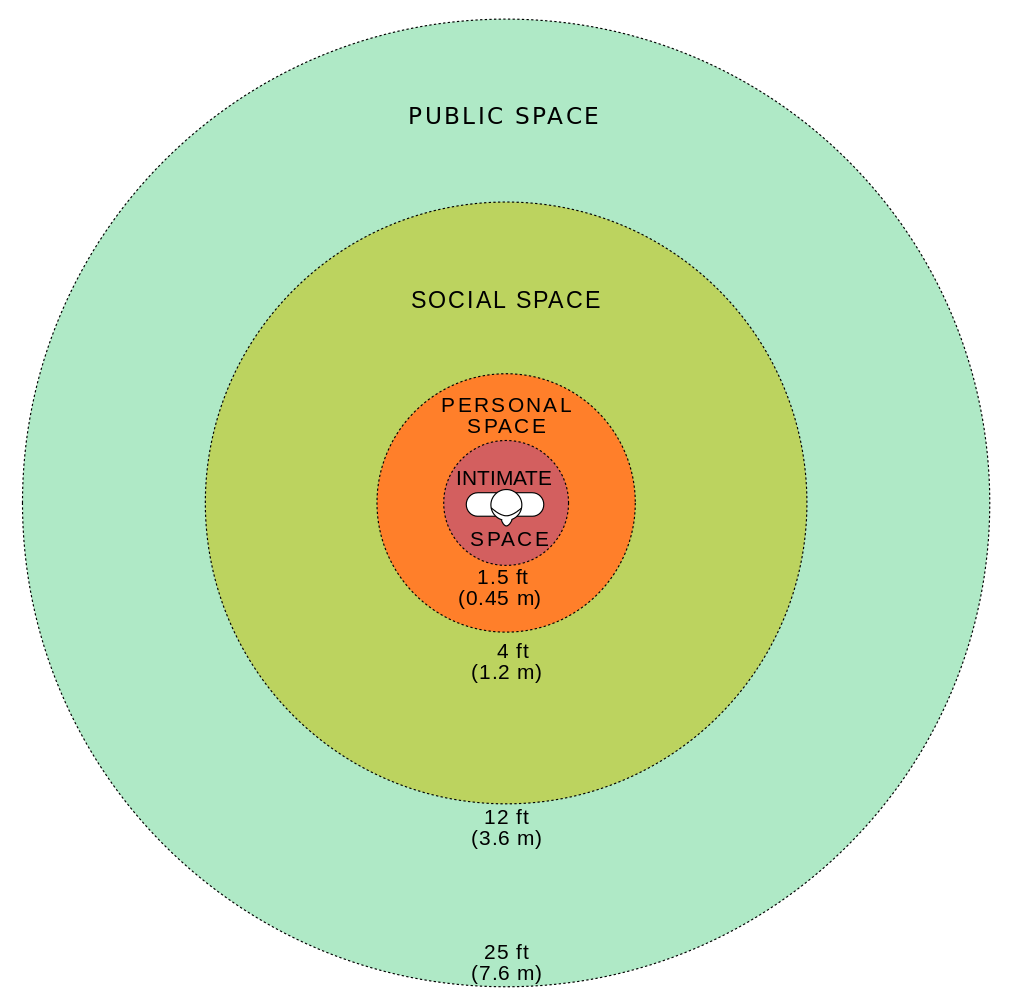
\includegraphics[width=0.75\textwidth]{figures/hall.png}
   \caption{The 4 different zones/phases of a distancing chart made by Edward t. Hall, to measure different comfort zones \cite{Hall}}
    \label{fig:hall}
\end{figure}

The personal space has been heard of before as a intimate space belonging to the person inside that zone, this is psychologically considered theirs. Entering this space is considered intimate and is not desired from a robot used to guide people around. However, it would be likeable to minimum enter the social zone. This zone is where it is described as likeable to enter a conversation with another person due to the safe distancing to the person and normally when following a person this zone would be optimal as well. And the public zone is a zone where people will most likely ignore the fact that the robot is trying to communicate with them, so to conclude - with Hall's model of interpersonal spacing the most desirable comfort zone the robot should operate in is the social zone, which is described as 1.2m as the "close-zone". Small deviations into the public zone will likely occur when the person guided is following the robot \cite{Hall}.\\

Another model is the \textit{Compensation model} this is not defined by space, like Hall's model, but rather suggesting non-verbal equilibrium between two persons. This means that when e.g. person A increase closeness in form of keeping eye contact, then the likeable other, person B, should compensate for this increase by decreasing the closeness by averting his/her gaze, or physically distancing themselves to person A. This can be used as a guideline for human-robot interaction so that sensors alert the system when noticing some of these cues.\\
Elaborating on the research in the paper this project deduced that a model was derived from the research on nonverbal cues, that described that the person will have to distance themselves to the robot, if the robot kept maintaining eye contact. Another model is proposed called the \textit{attraction-transformation model}, to connect the verbal and nonverbal cues,to avoid people disliking the robot due to disruption of the personal space.\\
\\
A resemblance can be seen between non-verbal contact and likeness of the robot. If the person has prejudices about a certain robot, averting its eyes can be a good response, because then the person will not feel as if they interact with it on a personal level. A way to avoid this is to either follow these guidelines or design a robot that has no close relation to a human being, because a human wont perceive a metal arm the same way as they perceive a human-like robot. However, it is important to have a robot with close human resemblance (but not too much) for the user to feel more secure \cite{mumm2011human}, e.g. \textit{Telenoid}, as seen in figure \ref{fig:telenoid} and figure \ref{fig:telenoid2}.

\begin{figure}[H]
    \begin{minipage}[b]{0.36\linewidth}
        \centering
    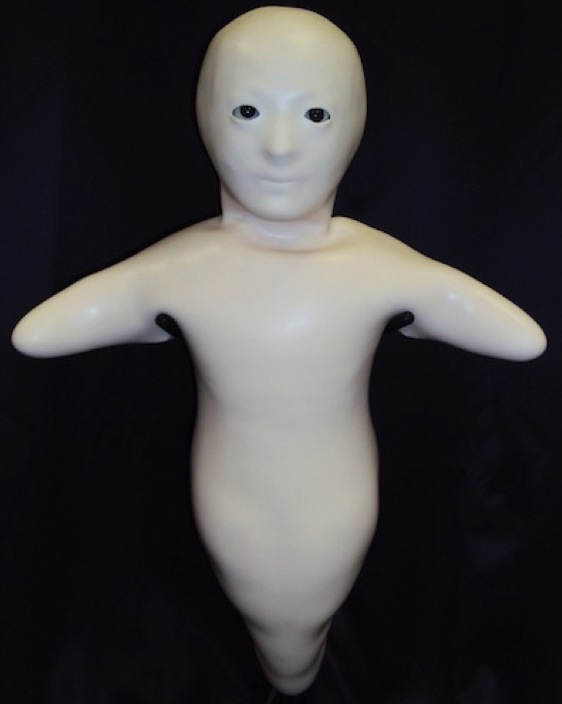
\includegraphics[width=\textwidth]{figures/telenoid.jpeg}
    \caption{A social robot, Telenoid R1 by Hiroshi Ishiguro\cite{telenoidIMG}.}
    \label{fig:telenoid}
    \end{minipage}
        \hspace{0.2cm}
    \begin{minipage}[b]{0.60\linewidth}
        \centering
        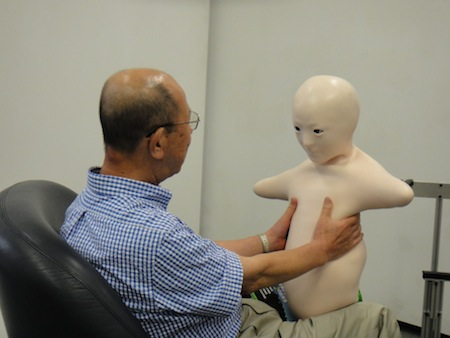
\includegraphics[width=\textwidth]{figures/telenoid2.jpeg}
        \caption{A man holding and interacting with the Telenoid robot\cite{telenoidIMG}.}
        \label{fig:telenoid2}
    \end{minipage}
\end{figure}

The uncanny valley illustration describes the aforementioned statement, that the likeness of a human being can be advised against, as seen in figure \ref{fig:uncanny}.

\begin{figure}[H]
    \centering
    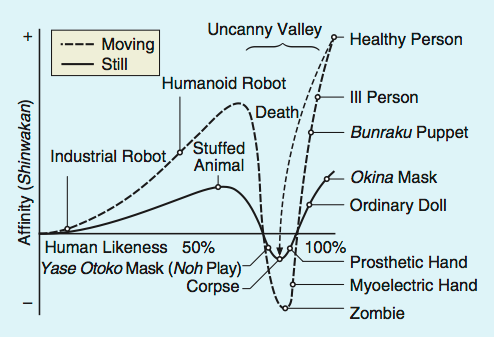
\includegraphics[width=.75\textwidth]{figures/uncannyvalley.png}
    \caption{Uncanny valley graph, is a model, that describe the humans reaction to an industrial robot manipulator, a robot like wall-E, almost human like to a perfect human robot. If the robot falls into almost human-like it falls into the uncanny valley, it looks like a person, but the movement might be putting people off because of the resemblance to a walking dead 
    \cite{mori2012uncanny}.}
    \label{fig:uncanny}
\end{figure}

It can be seen that when closing in on 100\% human likeness the affinity drops to a negative effect and people starts feeling it is wrong. 
Presenting movement will change the graph immensely, because the object will be approximating our movements and a connection towards the moving object is established, however it can change the graph for the worse as well, especially when the robot is very close to human likeness - then it feels more like a walking dead rather than a comfortable being.\\
When designing a robot it is clear that the social robot must not fall into this valley, else it will have the opposite effect of what is wanted, such as familiarity and good connections to the person it is servicing.
Since the robot is moving but is not alive it must not resemble a human too much, else it will be associated with something horrible like a zombie.\\